\documentclass{llncs}
\usepackage{graphicx}
\usepackage{booktabs}
\usepackage{amsmath}
\usepackage{hyperref}

\setlength{\textfloatsep}{6pt plus 1pt minus 2pt}
\setlength{\intextsep}{4pt plus 1pt minus 2pt}
\setlength{\abovecaptionskip}{3pt}
\setlength{\belowcaptionskip}{1pt}
\renewcommand{\arraystretch}{0.9}

\begin{document}

\title{An Alignment Check for Debiasing Corrections: A Negative-Control Case Study in Drug Repurposing}

\author{Rishik Kondadadi\inst{1} \and John Ortega\inst{2}}
\institute{University of Minnesota \and Northeastern University}

\maketitle

\begin{abstract}
A bias-diagnostic metric can judge a debiasing correction only if it is sensitive to what that correction changes; two corrections with different mechanisms can target different quantities, and a metric tuned to one will misjudge the other regardless of which is substantively better. We formalize this as an alignment check: score each correction's own penalty term as a standalone classifier of whatever the bias metric flags, and treat near-chance AUROC as evidence the metric cannot see that mechanism at all. We develop the check through a case study in drug repurposing, where a model trained to rank candidates for one indication also learns what is shared across drugs on the same organ system; in our data the convulsant bemegride ranks first among non-antiepileptic candidates for epilepsy. We test two corrections for this confound, naive area-score subtraction and a negative-control method adapted from genomics and pharmacoepidemiology, across five indications. Naive wins every bias-diagnostic metric measured. Computing the principled method's penalty term correctly for held-out compounds, an out-of-sample estimate an earlier version of this analysis silently zeroed instead of computing, changes the picture: the term stays near chance for depression, antipsychotic, and lipid, matching a direct intervention test that dials each correction's real effect into the score and finds the bias metrics genuinely unmoved by the principled method there; for epilepsy, our own motivating case, it does not, and a smaller but real response appears under the same intervention. A synthetic experiment with a known ground-truth confound explains both outcomes with one mechanism: the principled method's factor recovers the true confound better than naive's own penalty does (0.83 vs.\ 0.68 AUROC against ground truth), yet projecting it out of the final score, the method's actual correction step, does not reduce its presence in the ranked list, while naive's cruder subtraction does. The method identifies the confound; the specific way it is applied does not act on what it identifies, a distinct and more general finding than metric blindness.
\end{abstract}

\section{Introduction}

A bias-diagnostic metric is itself a measurement, and a measurement has a detection limit. When two debiasing corrections are compared against one bias metric and one wins, the usual reading is that the winning correction removes the bias better. A second reading is available whenever the two work through different mechanisms: the metric may simply be built to see one and not the other, in which case the comparison never tested what it looked like it was testing. Telling these readings apart requires checking, directly, whether the metric could have detected the losing correction's effect at all, rather than inferring quality from the scoreboard alone. We call this an alignment check: score each correction's own penalty term, the quantity it subtracts or projects out, as a standalone classifier of whatever the metric flags. A term that classifies the flag near chance is one the metric cannot reward or penalize, independent of correction quality.

We develop this check through a case study chosen because it produces exactly the puzzle the check is built to resolve. Chemical structure is not the only thing a repurposing model can learn to exploit: a model trained to separate antiepileptic drugs from everything else also, incidentally, learns what distinguishes neurology drugs from the rest of the pharmacopeia, and that second signal rides along with the first. In a plain ECFP4 fingerprint model trained on known antiepileptic drugs, bemegride, a convulsant once used to induce seizures for electroconvulsive therapy, ranks first among 1{,}522 non-antiepileptic candidates, ahead of every genuinely plausible lead. We reproduce this exactly (score 0.7942, matching a prior run) as this paper's motivating case. A companion study from this group audited evaluation-protocol choices in LINCS-based repurposing models and reported this same ranking~\cite{kondadadi2026ichiaudit}; it proposes no model and leaves correction methods to future work.

The same pattern appears in aggregate. Restricting to drugs with a WHO ATC classification, nervous-system drugs make up 18.8\% of the top 50 false positives for a depression model and 15.2\% for an antipsychotic model, against base rates of 10.2\% and 10.6\%, 1.5 to 1.8 times base rate, smaller than a name-matched Hub label had suggested; ATC covers only 9.7\% of the LINCS library, mostly marketed drugs, used throughout.

\begin{figure}[t]
\centering
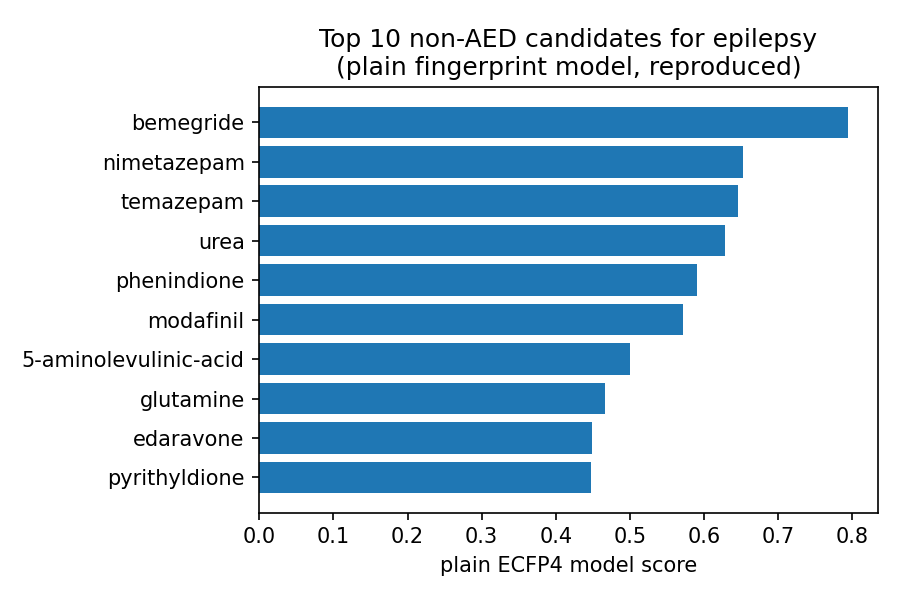
\includegraphics[width=0.48\textwidth]{fig1_bemegride_top10.png}
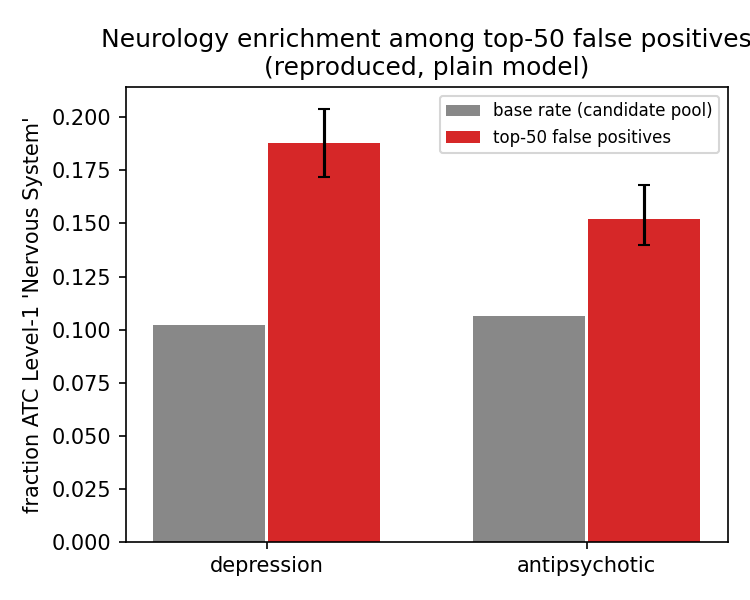
\includegraphics[width=0.48\textwidth]{fig1_neurology_enrichment.png}
\caption{Left: top 10 non-antiepileptic candidates ranked by a plain ECFP4 model; bemegride, a convulsant, ranks first. Right: nervous-system drugs (ATC 'N') enriched among top-50 false positives of depression/antipsychotic models vs.\ base rate.}
\label{fig:motivation}
\end{figure}

Two corrections suggest themselves. The simple one subtracts a generic area score from the disease-specific score, directly penalizing confounded-class membership; prior informal analysis assumed this collapses precision too far to use. The more principled one borrows an idea from genomics and pharmacoepidemiology: estimate the shared organ-system factor from negative-control indications, diseases in the same area treated by a different mechanism, and remove only that factor rather than a blunt membership score. We built and evaluated it. It did not beat the simple one on any bias-diagnostic metric measured, which is where this paper could have stopped and reported a negative result.

Instead we apply the alignment check, and it complicates the conclusion rather than resolving it. Section~\ref{sec:alignment} shows the bias metrics' flags are predictable from the same base representation for three of five targets but not uniformly, and a direct intervention test (Section~\ref{sec:intervention}) confirms the metric is genuinely insensitive to the principled method there, with a real, smaller exception for epilepsy. A synthetic experiment with a known confound (Section~\ref{sec:synthetic}) explains why: the method's own factor recovers the true confound better than naive's penalty does, but how it is applied, fit jointly then projected out at scoring, does not reduce the confound's presence in the ranking the way naive's cruder subtraction does. Table~\ref{tab:main-bias}'s comparison is real; the reason is closer to a correction-application gap than to the metric being blind to the mechanism.

\section{Related Work}
\label{sec:related}

\paragraph{Negative controls for unwanted variation.}
RUV via negative controls is an established genomics technique: RUV-2~\cite{gagnonbartsch2012ruv} estimates latent confounding factors from known-null control genes and removes them before testing; later work~\cite{gerard2021ruvstar} unifies several RUV variants in one framework. Surrogate variable analysis~\cite{leek2007sva} and empirical-Bayes batch correction~\cite{johnson2007combat} address related but distinct versions; ComBat needs known batch labels rather than negative controls, why we follow the negative-control strategy. Negative-control exposures/outcomes in pharmacoepidemiology~\cite{lipsitch2010negativecontrols} formalize the same logic for drug-effect confounding, in active use~\cite{negctrlreview2023}. Our area-factor step is a direct structural analogue, applied to indications rather than genes.

\paragraph{Debiasing drug-repurposing and DTI models.}
NRBdMF~\cite{azuma2022nrbdmf} factorizes a signed drug$\times$disease matrix from SIDER~\cite{kuhn2016sider} to reduce false positives through within-drug directionality; it never uses other diseases as negative controls, so we include it as a baseline. TAPB~\cite{tapb2025b} and DRDM~\cite{meng2025drdmb} address other biases (target-popularity, graph-degree); neither targets organ-system confounding. Campillos et al.~\cite{campillos2008sideeffect,kuhn2010sider} first showed SIDER-derived phenotypic similarity carries repositioning signal, the basis for our hard negatives.

\paragraph{Benchmarks and resources.}
repoDB~\cite{brown2017repodb} provides a curated gold-standard set of approved/failed drug-disease pairs, a standard secondary comparison point. The Drug Repurposing Hub~\cite{corsello2017repurposinghubb}, a name-matched label used in prior work from this group, has limited coverage; we replace it with ATC classification. Epileptogenic/proconvulsant lists have an established clinical literature base~\cite{ruffmann2006epileptogenic,chen2016druginducedseizures,shorvon2002proconvulsant}.

\paragraph{Validity of bias-evaluation metrics.}
A smaller literature asks whether a protocol can detect what it claims to measure: scaffold splits overestimate performance relative to a realistic split~\cite{scaffoldsplits2024}, and affinity benchmarks reward memorization unless reweighted~\cite{similarityaware2025}. Neither originates in computational biology. Ours is more specific: whether a bias-diagnostic metric can see a correction's mechanism at all.

\section{Data}
\label{sec:data}
We build on the nine ChEMBL~\cite{zdrazil2024chemblb} indication classes used in our companion study (epilepsy, depression, antipsychotics, antibacterials, antidiabetics, antineoplastics, lipid-lowering drugs, NSAIDs, betablockers as an antihypertensive proxy), over the same 9{,}878-compound LINCS library, extended with nine further ATC-defined indications (Parkinson's disease, anxiolytics, antidementia drugs, opioid analgesics, renin-angiotensin antihypertensives, antacids, osteoporosis drugs, antimycotics, immunosuppressants) chosen so every original class has at least one same-area, different-mechanism negative-control partner. ATC Level-1 codes come from the ChEMBL molecule API by full InChIKey; only 954 of 9{,}878 compounds (9.7\%) carry any ATC classification, most of the library being research/tool compounds, not marketed drugs, why Section~\ref{sec:intro-confound}'s enrichment is smaller than a name-matched Hub label had suggested.

SIDER~\cite{kuhn2016sider} side-effect data is joined by PubChem CID, extending a prior join covering only 1{,}725 compounds. Coverage remains low, 543 of 9{,}878 (5.5\%), for the same reason as ATC. We use its characteristic adverse-effect terms as hard negatives (convulsion-family for epilepsy, hypotension for antihypertensives, hyperglycaemia for antidiabetics) where such a term map makes sense, not inventing one otherwise.

For epilepsy, we use a 43-drug proconvulsant list from this group's own prior, unpublished work, stated plainly rather than as an external resource: literature-curated from Chen, Albertson \& Olson~\cite{chen2016druginducedseizures}, a peer-reviewed review of drug-induced seizures, cross-validated against two public sources. Of 82 canonical compounds, 62 resolve to a compound in our library; of those, 38 (61\%) carry a SIDER-listed convulsion/seizure adverse effect, and 24 (39\%) match a risk tier in the independently published systematic review of Ruffmann, Bogliun \& Beghi~\cite{ruffmann2006epileptogenic}, a substantial overlap given SIDER's own sparse 5.5\% coverage.

\section{Method}
\label{sec:method}
Each compound is represented by concatenating a 32-component PCA of its ECFP4 fingerprint (TruncatedSVD, no indication-matrix leakage) with a 16-dim embedding from a free logistic matrix factorization fit jointly across all 18 indications. Chemistry is necessary, not cosmetic: a pure co-occurrence factorization carries almost no signal here, 94\% of the library has zero positive indications and per-indication training AUPRC is indistinguishable from base rate, why NRLMF/NRBdMF add drug or disease similarity rather than the interaction matrix alone; we add chemistry for the same reason.

On top of this representation we compare four scorings for target indication $k_0$. \emph{Plain} fits one logistic regression per indication, no area correction. \emph{Naive subtraction} scores the plain score minus $\lambda$ times a min-max-normalized mean indication rate over $k_0$'s negative-control set, $\lambda=2$. \emph{NRBdMF} factorizes a signed drug-by-disease matrix~\cite{azuma2022nrbdmf}: $-1$ ChEMBL/ATC indication, $+1$ SIDER adverse-effect hit, chemistry withheld, matching the original specification. \emph{Proposed}: for $k_0$'s negative-control set $\mathrm{NC}(k_0)$, same ATC area, different mechanism, take the train-only residuals of the already-fit plain models on $\mathrm{NC}(k_0)$'s columns, their leading left singular vectors as area factor $A$ (Gagnon-Bartsch and Speed's RUV-2 strategy~\cite{gagnonbartsch2012ruv}, applied to indications rather than genes), refit $k_0$ with $[\text{chemistry+MF}, A]$, score with $A$'s coefficients dropped.

We later tested a shrunk version of this correction, scaling $A$ by $s\in[0,1]$ following Gerard and Stephens' unified RUV family~\cite{gerard2021ruvstar}; Section~\ref{sec:shrinkage} reports no improvement.

\subsection{The alignment check}
\label{sec:alignment-check}
Any correction scoring a candidate as a base score minus (or plus) a penalty term, naive subtraction's $\lambda$-weighted area rate and the proposed method's projected-out $A$-coefficients both have this form, can be probed independently of whatever metric judges it. Given a bias-diagnostic metric defined through a binary flag $F$ (same-area membership, hard-negative membership, or any other criterion the metric penalizes), the check scores the correction's own penalty term $P$ as a standalone classifier of $F$ via $\mathrm{AUROC}(P,F)$. Near-0.5 AUROC means $P$ carries no information about $F$: the metric cannot reward or penalize that mechanism regardless of correction quality, so a comparison against a baseline whose term \emph{is} informative about $F$ is not on equal footing. We apply this to our two corrections in Section~\ref{sec:alignment}; the check names no drug-repurposing-specific quantity.

Section~\ref{sec:alignment}'s result has a structural reason. \textbf{Proposition.} Let $X$ be the shared representation on which every negative-control indication's model is fit by $L_2$-penalized logistic regression at inverse-strength $C$ (weights $W$), coefficients $\hat\beta_j$, fitted probabilities $\hat P$, train rows only. Each residual $r_j = y_j - \hat p_j$ satisfies $X_{\mathrm{tr}}^\top W r_j = \hat\beta_j / C$: orthogonality to $X$ is exact only as $C \to \infty$; at finite $C$ the deviation is proportional to $\hat\beta_j$, not zero. $A$, the leading left singular vectors of $R=[r_1,\dots,r_{|\mathrm{NC}|}]$, inherits whatever orthogonality $R$ has.

We measured this rather than assuming it away: at the $C=1$ used throughout, $A$'s projection onto $X$'s column space holds 34--40\% of $A$'s variance, not the near-zero a pure guarantee would give; the genomics domain's unregularized OLS fit (Section~\ref{sec:ruv-generalization}) is where the exact case holds. Section~\ref{sec:alignment} tests both halves empirically.

\section{Experiments}
\label{sec:experiments}

\subsection{Reproducing the motivating confound}
\label{sec:intro-confound}
We retrained the plain ECFP4 model for epilepsy, depression, and antipsychotics, averaged over five seeds, confirming both parts of Section~1's motivating observation: bemegride ranks first of 1{,}522 non-antiepileptic candidates, matching the pre-existing score, and the top-50 false positives for depression and antipsychotic models are enriched for nervous-system drugs 1.5 to 1.8 times each pool's base rate (18.8\% vs.\ 10.2\%, 15.2\% vs.\ 10.6\%). We looked for, but could not locate in any saved script, the specific AUPRC collapse from 0.45 to 0.17 an earlier informal analysis attributed to naive area-score subtraction; we report what we can actually measure instead.

\subsection{Evaluation protocol}
We evaluate under three cross-validation schemes from the matrix-factorization repurposing literature: CVS1, a random 20\% cell holdout; CVS2, a cold-start-drug holdout of 20\% of compounds; CVS3, a cold-start-disease holdout of the entire target column. Each scheme runs five times with independent splits on an identical 1{,}702-compound pool shared by all four methods. A scaffold-disjoint CVS2 variant is also in the repository, since a random compound holdout can still leak near-duplicate scaffolds.

\subsection{Main results}
Table~\ref{tab:main-auprc} reports CVS2 AUPRC on the true indication label (CVS1 and CVS3 tables, same pattern, are in the repository); Table~\ref{tab:main-bias} reports the two bias-diagnostic metrics that matter most here, the same-ATC-area rate among the top 50 false positives and the median rank percentile of SIDER-flagged hard negatives.

\begin{table}[t]
\centering
\small
\caption{AUPRC on true indications, CVS2 (mean over 5 reruns; 95\% bootstrap CI in parentheses).}
\label{tab:main-auprc}
\begin{tabular}{lcccc}
\toprule
Target & Plain & Naive subtract & NRBdMF & Proposed \\
\midrule
depression & 0.201 (.114,.289) & 0.190 (.105,.262) & 0.039 & 0.181 (.112,.247) \\
antipsychotic & 0.440 (.252,.628) & 0.412 (.215,.608) & 0.039 & 0.437 (.264,.611) \\
epilepsy & 0.091 (.065,.127) & 0.090 (.067,.128) & 0.024 & 0.085 (.065,.112) \\
\bottomrule
\end{tabular}
\end{table}

\begin{table}[t]
\centering
\small
\caption{Bias-diagnostic metrics. Top-50 same-area rate: lower is better (base rate $\approx$ 0.09--0.11). Hard-negative/proconvulsant rank: higher percentile is better.}
\label{tab:main-bias}
\begin{tabular}{llcccc}
\toprule
Metric / Target & CVS & Plain & Naive subtract & NRBdMF & Proposed \\
\midrule
area rate, depression & 2 & 0.112 & 0.024 & 0.084 & 0.112 \\
area rate, antipsychotic & 2 & 0.136 & 0.096 & 0.084 & 0.144 \\
area rate, epilepsy & 2 & 0.144 & 0.068 & 0.120 & 0.176 \\
hard-neg.\ pct., epilepsy & 2 & 38.4 & 50.9 & 47.8 & 42.0 \\
proconv.\ pct., epilepsy & 2 & 30.9 & 71.8 & 49.2 & 26.3 \\
\bottomrule
\end{tabular}
\end{table}

Four things stand out. NRBdMF performs close to chance everywhere (AUPRC 0.02 to 0.15), confirming what the matrix diagnostics already suggested: a pure within-drug signed factorization, no chemistry, has little to work with on an 18-indication matrix this sparse. The proposed method tracks plain closely on AUPRC, the precision-preservation property it was designed for, but on the depression/antipsychotic/epilepsy bias metrics in Table~\ref{tab:main-bias} it is dominated by naive subtraction, often by a wide margin; the clearest case is the proconvulsant panel, where naive pushes it from the 31st percentile to the 72nd while proposed moves it under 5 points, and in the epilepsy CVS2 row in the wrong direction. Contrary to this paper's own motivating assumption, naive subtraction's AUPRC cost is modest across every row measured under all three CVS schemes, never approaching the 62\% relative collapse an earlier informal analysis had reported. Betablocker and lipid, a different same-area pair, split: betablocker shows almost no method differentiation (AUPRC within 0.01 of plain, area rate 0.108 to 0.112), lipid reproduces the core pattern (naive halves the area rate, 0.104 to 0.052, at no AUPRC cost; proposed moves neither). The divergence generalizes to one of two pairs tried beyond the original three. A reconstructed DRDM baseline (no public code or full text exists, Section~\ref{sec:related}) behaves like plain throughout, consistent with targeting a different bias.

\subsection{Negative-control validity check}
A method that identifies an area factor from negative controls should, if those controls are mechanistically independent, leave each control's predictability roughly unchanged when corrected using a factor from the \emph{other} controls. We ran this leave-one-negative-control-out diagnostic for every (target, control) pair; 13 of 14 cells cluster within $\pm0.03$ of zero AUPRC change, consistent with, though not sufficient on its own to prove, independence. The exception, anxiolytic, showed a large positive delta at 4-5 reruns ($+0.127$, $+0.126$) but also the largest std by far; 20 seeds shrank the mean to $+0.034$, within 1 SE of zero ($0.129/\sqrt{15}=0.033$), small-sample noise from anxiolytic's 7-positive class, not a calibration failure.

\subsection{Shrinkage follow-up}
\label{sec:shrinkage}
The most natural explanation for Table~\ref{tab:main-bias} is that the negative-control classes are small, 4 to 21 positives each, and the resulting area factor is mostly noise. We tested this with empirical-Bayes-style shrinkage of the factor: $A \leftarrow sA$ for $s \in \{0, 0.25, 0.5, 0.75, 1.0\}$, selecting $s$ via the same leave-one-negative-control-out diagnostic. It selected full-strength, unshrunk correction ($s=1$) for all three targets, statistically indistinguishable from the original, ruling out noisy estimation. An RUV-4-style joint alternating estimator, re-estimating the factor and controls' fits together, did not beat naive subtraction either, and shows the same near-chance alignment signature (\url{results/ruv4_alignment_check.csv}), so the account holds under a mechanistically distinct strategy too.

\subsection{Testing the identifiability-violation hypothesis directly}
\label{sec:overlap}
RUV's own identifying assumption~\cite{gerard2021ruvstar} is that a negative-control column must carry zero loading on the covariate of interest; if that fails, the area factor would absorb target signal, costing real precision along with the confound. We regressed the target's true label, train rows only, onto its fitted area factor and measured $R^2$, which should sit near zero under the assumption. All six cells are small, 0.0006 to 0.021, and do not track naive's advantage: epilepsy has the smallest overlap but the largest gap in naive's favor, the opposite of what the hypothesis predicts. This rules it out.

\subsection{Applying the alignment check}
\label{sec:alignment}
Ruling out identifiability leaves a more mundane candidate: the bias metrics may sit closer to what naive directly penalizes, raw negative-control membership, than to proposed's residualized factor. We apply the alignment check (Section~\ref{sec:alignment-check}): for each target, under CVS2, compute naive's penalty term and proposed's term made concrete (the contribution $A$'s coefficients would have made had they not been projected out) for every non-indicated test compound, and score each as a classifier of the exact compounds the bias metrics flag: same-ATC-area, SIDER-hard-negative, or proconvulsant-panel membership.

\begin{table}[t]
\centering
\small
\caption{AUROC of each method's penalty term, and of $X$ alone, as a classifier of the flagged compounds (mean, 5 seeds, CVS2). 0.5 = no information. Proposed's term uses the out-of-sample estimate (Section~\ref{sec:oos-fix}); its sign is arbitrary (an SVD factor), so values are sign-free, $\max(\mathrm{AUROC},1-\mathrm{AUROC})$.}
\label{tab:alignment}
\begin{tabular}{llccc}
\toprule
Target & Flag & Naive's term & Proposed's term & $X$ alone \\
\midrule
depression & same-ATC-area & 0.766 & 0.517 & 0.718 \\
depression & hard-negative & 0.636 & 0.508 & 0.514 \\
antipsychotic & same-ATC-area & 0.774 & 0.516 & 0.706 \\
antipsychotic & hard-negative & 0.663 & 0.502 & 0.591 \\
epilepsy & same-ATC-area & 0.787 & 0.657 & 0.722 \\
epilepsy & hard-negative & 0.600 & 0.565 & 0.613 \\
epilepsy & proconvulsant & 0.721 & 0.676 & 0.695 \\
\bottomrule
\end{tabular}
\end{table}

\label{sec:oos-fix}
An earlier version of this table scored test rows using the SVD's own output directly, exactly zero there by construction (a zero residual row forced by the negative controls' own train mask, $\sim10^{-16}$): the original "0.50 AUROC" was the AUROC of a value mathematically zero for every test compound, not a property of the method. We instead fit a linear out-of-sample projection from $X$ to the train rows' own factor values (5-fold CV $R^2$ 0.44--0.56, non-degenerate) for test rows below.

Naive's term separates every flag well above chance, 0.60 to 0.79, unaffected by this fix. The corrected proposed term stays near chance for depression and antipsychotic, 0.502 to 0.517, the original claim holding once computed correctly. It does not for epilepsy, 0.56 to 0.68: the correction's own dropped factor carries real information about the flagged compounds, in this paper's own motivating case. By the Proposition, proposed's term is only partially orthogonal, on train rows, to representation $X$; the rightmost column tests, rather than assumes, whether $F$ is predictable from $X$. Same-ATC-area is well predicted by $X$ on every target, 0.706 to 0.722, close to naive's own 0.766 to 0.787: most of what marks a compound as belonging to the confounded area is already present in $X$ before any negative-control information is added. This does not explain why epilepsy's term specifically carries signal while depression's and antipsychotic's do not; Section~\ref{sec:synthetic} does.

This two-step recipe, orthogonality by construction plus an empirical flag-predictability check, names nothing drug-repurposing-specific and applies wherever a residualized correction meets a membership-based bias metric. It is a diagnostic of statistical association, not of what the metric does when the real effect is applied; Section~\ref{sec:intervention} tests that directly.

\label{sec:ruv-generalization}
We also re-ran this check outside drug repurposing, on the dataset RUV-2 was introduced on: Vawter et al.'s brain gene-expression study~\cite{vawter2004gender}, gender as the factor of interest, lab as the confound, and Gagnon-Bartsch and Speed's 799 housekeeping controls~\cite{eisenberg2003housekeeping}. Step one holds exactly: each control gene's OLS residual on gender satisfies the normal equations to floating-point precision, so $A$'s genomics analog is exactly orthogonal to gender. Step two differs: lab is not predictable from gender (AUROC 0.39--0.41, near or below chance), unlike same-ATC-area membership above. As predicted, the orthogonalized factor stays informative about lab (0.50--0.94 alone, 0.95--1.00 combined), matching or beating naive's unprojected summary (0.55--0.76): the two domains diverge exactly where the check predicts. Donor-grouped CV leaves the combined read unchanged (0.95--1.00); the gender-predicts-lab baseline moves from 0.39--0.41 to 0.50--0.51, still at or below chance.

A third, harder domain: bladderbatch~\cite{dyrskjot2004bladder,leek2010batcheffects}, a 3-level cancer-status factor fit by ridge regression against a 5-level batch confound (57 samples, one level $n=4$, a thin base). Step one again holds exactly by the normal equation. Step two differs: cancer predicts batch moderately (0.722), yet the orthogonalized factor stays as informative about batch as naive's raw mean, or more so (0.68 against 0.62), not falling to chance, likely because $X$'s 2 columns are too low-dimensional to absorb batch's variance at moderate correlation. This refines, rather than confirms, the check's second step: predictability of $F$ from $X$ matters less than whether $X$ is rich enough to exhaust it.

\subsection{Confirming it directly: intervention, and a synthetic ground truth}
\label{sec:intervention}
Standalone AUROC does not show whether Table~\ref{tab:main-bias}'s metric actually moves when a penalty's real effect is dosed into the score. We sweep how much of each penalty is included, $\alpha\in\{0,0.25,0.5,0.75,1\}$ ($\alpha=1$ for naive and $\alpha=0$ for proposed reproduce Table~\ref{tab:main-bias}), and recompute the bias metrics at each dose, same CVS2 split, all five targets. Naive's metrics move strongly and monotonically for depression, antipsychotic, and lipid (epilepsy proconvulsant percentile: 30.9 at $\alpha=0$ to 71.8 at $\alpha=1$); proposed's stay exactly flat for the same three (depression area rate 0.112, lipid 0.104, throughout). Betablocker moves little under either, uninformative either way. Epilepsy again exceptions: proposed's metrics move a small real amount (area rate 0.180 to 0.140, proconvulsant percentile 26.4 to 32.7), a quarter naive's swing. This confirms the alignment claim operationally for three of five targets and the same exception as Table~\ref{tab:alignment}.

\label{sec:synthetic}
A real-data flag is a proxy; the true confound is unobserved. A simulation fixes that: 3{,}000 compounds, chemistry $X$, an organ-area confound $z$ itself a noisy function of a chemistry subspace, indication log-odds combining a disease-specific term with, for same-area diseases, $z$; negative controls share the area with an independently drawn mechanism. Over 5 seeds, AUPRC (0.483/0.302/0.482 plain/naive/proposed) reproduces Table~\ref{tab:main-auprc}'s pattern, and the top-50 rate of \emph{true} high-confound compounds (base rate 0.28) is 0.656/0.480/0.676: naive substantially reduces the real confound's presence in the ranking, proposed does not reduce it at all. Yet proposed's factor's AUROC against the true confound is 0.83, against naive's own 0.68: it identifies the real confound better, but projecting it out at scoring, its actual correction step, does not act on what it identified. One mechanism covers both findings above: where the factor carries little real signal (depression, antipsychotic, lipid) there is little for this gap to act on; where it does (epilepsy), the gap becomes the small effect just measured.

\section{Discussion and Limitations}
This paper set out to build a more principled alternative to a correction assumed too costly to use; naive won every bias metric measured, and we asked whether that scoreboard meant what it appeared to. The honest answer is target-dependent. For depression, antipsychotic, and lipid, the corrected check and the intervention test agree the metric genuinely cannot see the proposed method's mechanism; for epilepsy it partially can. Section~\ref{sec:synthetic}'s mechanism explains both: proposed's factor identifies the true confound well, better than naive's own penalty, but projecting it out, as the correction does, does not reduce the confound's presence in the ranking, while naive's subtraction does. Where the factor carries little leftover signal after $X$ already explains the flag, the gap is invisible; where it carries real signal (epilepsy), it becomes the small response found above.

We think the check, and the correction-application gap, are the more durable contributions, with a caveat learned the hard way once already: a bug zeroed the correction's out-of-sample factor for every held-out compound until this revision (Section~\ref{sec:oos-fix}), a cleaner "0.50 everywhere" result than the method earns. Identifying a confound correctly~\cite{gagnonbartsch2012ruv,gerard2021ruvstar,leek2007sva,lipsitch2010negativecontrols,negctrlreview2023} does not guarantee fit-then-project-out removes it from a ranked list. NRBdMF~\cite{azuma2022nrbdmf} runs chemistry-withheld, so its near-floor AUPRC reflects weak co-occurrence signal and has no residualized term; the check does not apply. DRDM~\cite{meng2025drdmb} has no public code or text; its baseline here is a reconstruction, not a verified reproduction.

Limitations: the check spans three domains, the third partial. ATC/SIDER cover under 10\% of the library. CVS3 collapses plain and proposed together. repoDB~\cite{brown2017repodb} gives 82--91\% label agreement for three targets, too little overlap for an AUPRC check. Code: \url{https://github.com/edanmn/area-debiasing-drug-repurposing}.

\bibliographystyle{splncs04}
\bibliography{refs}

\end{document}
